\documentclass{article}

\usepackage[final]{style}
\usepackage[utf8]{inputenc} % allow utf-8 input
\usepackage[T1]{fontenc}    % use 8-bit T1 fonts
\usepackage{hyperref}       % hyperlinks
\usepackage{url}            % simple URL typesetting
\usepackage{booktabs}       % professional-quality tables
\usepackage{amsfonts}       % blackboard math symbols
\usepackage{nicefrac}       % compact symbols for 1/2, etc.
\usepackage{microtype}      % microtypography
\usepackage{verbatim}
\usepackage{graphicx}       % for figures

\title{Lecture \#14: Visual Bag of Words}

\author{
  Megha Srivastava, Jessica Taylor, Shubhang Desai, Samuel Premutico,  Zhefan Wang
  \\
  Department of Computer Science\\
  Stanford University\\
  Stanford, CA 94305 \\
  \texttt{\{meghas, jtaylor5, shubhang, samprem, zwang141,lbagdas\}@cs.stanford.edu} \\
}

\begin{document}

\maketitle


\section{Introduction}	
In this lecture, we learn another approach to recognition. To recognize objects in images, we need to first represent them in the form of feature vectors. Feature vectors are mathematical representations of an image's important features.  These feature vectors, for example, can be the raw color values of the image or contain information about the position of the pixel in the image as we have seen and implemented in Homework 5. We then create a space representation of the image to view the image values in a lower dimensional space.  Every image is then converted into a set of coefficients and projected into the PCA space.  The transformed data is classified using a classifier. Some examples of such classifiers include K-means and HAC.  This process of going from an image to a useful representation of the image in a lower dimensional space can be achieved in many ways.  In this lecture, we discuss another approach entitled Visual Bag of Words.

\subsection{Idea of Bag of Words}
The idea behind "Bag of Words" is a way to simplify object representation as a collection of their subparts for purposes such as classification. The model originated in natural language processing, where we consider texts such as documents, paragraphs, and sentences as collections of words - effectively "bags" of words. Consider a paragraph - a list of words and their frequencies can be considered a "bag of words" that represents the particular paragraph, which we can then use as a representation of the paragraph for tasks such as sentiment analysis, spam detection, and topic modeling. 

Although "Bag of Words" appears to be associated with language, the idea of simplifying complex objects into collections of their subparts can be extended to different types of objects. In Computer Vision, we can consider an \textbf{image} to be a \textbf{collection of image features}. By incorporating frequency counts of these features, we can apply the "Bag of Words" model towards images and use this for prediction tasks such as image classification and face detection.

There are two main steps for the "Bag of Words" method when applied to computer vision, and these will further be explored in the Outline section below. 

1. Build a "dictionary" or "vocabulary" of features across many images - what kinds of common features exist in images? We can consider, for example, color scheme of the room, parts of faces such as eyes, and different types of objects.

2. Given new images, represent them as histograms of the features we had collected - frequencies of the visual "words" in the vocabulary we have built. 
\subsection{Origins}
The origins of applying the "Bag of Words" model to images comes from Texture Recognition and, as previously mentioned, Document Representation. 

1. Textures consist of repeated elements, called textons - for example, a net consists of repeated holes and a brick wall consists of repeated brick pieces. If we were to consider each texton a feature, then each image could be represented as a histogram across these features - where the texton in the texture of the image would have high frequency in the histogram. Images with multiple textures, therefore, can be represented by histograms with high values for multiple features.  

2. Documents consist of words which can be considered their features. Thus, every document is represented by a histogram across the words in the dictionary - one would expect, for example, the document of George Bush's state of the union address in 2001 to contain high relative frequencies for "economy", "Iraq", "army", etc. 

Thus, a "bag of words" can be viewed as a histogram representing frequencies across a vocabulary developed over a set of images or documents - new data then can be represented with this model and used for prediction tasks. 

\section{Algorithm Summary}
Let's describe in detail how the Bag of Words algorithm can be applied to a large set of images.

\subsection{Extracting Interesting Features}
The first step in the Bag-of-Words algorithm is extracting the features of the images. We eventually use these features to find the most common features across our dataset of images. We can choose any type of feature we want to find our features. For example, we can simply split our images into a grid and grab the subimages as features (shown below). Or, we can use corner detection of SIFT features as our features.
\begin{center}
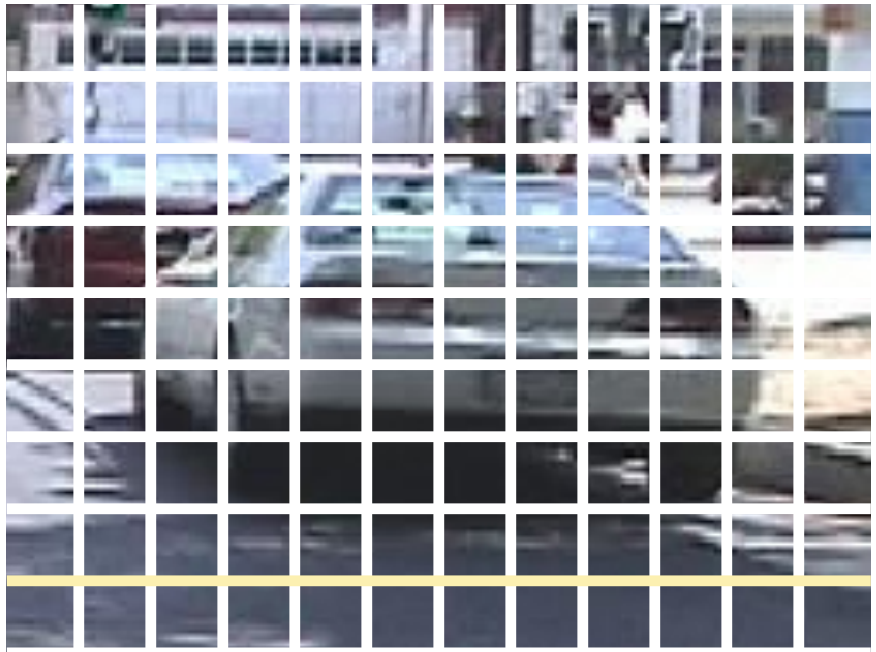
\includegraphics[scale=0.5]{grid_features.png}\\
Using grid of subimages as features \cite{slides}
\end{center}

\subsection{Learning Visual Vocabulary}
Once we have our features, we must turn this large feature set into a small set of "themes". These "themes" are analogous to the "words" in the Natural Language Processing version of the algorithm. As mentioned above, in the Computer Vision application, the "words" are called textons.

To find textons, we simply cluster our features. We can use any clustering technique (K-Means is most common, but Mean Shift or HAC may also work) to cluster the features. We then use the centers of each cluster as the textons. Our set of textons is known as a visual vocabulary. An example of a visual vocabulary is given below.
\begin{center}
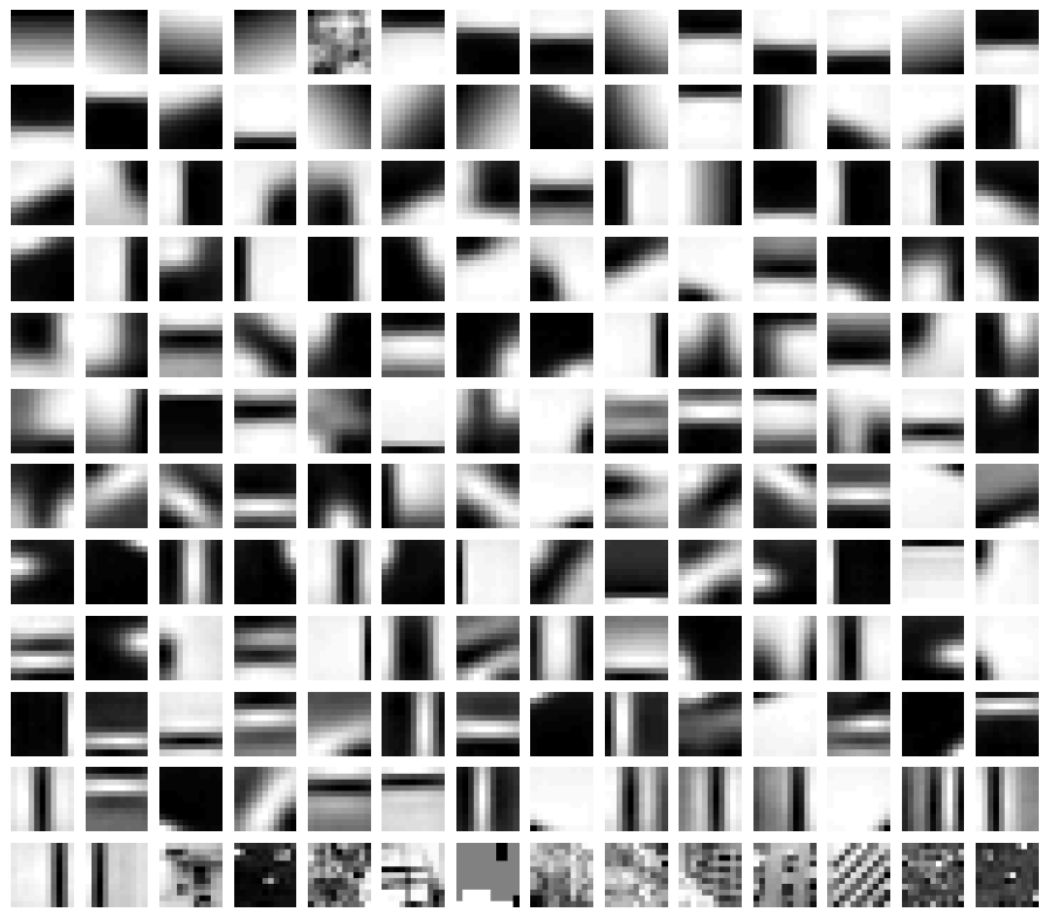
\includegraphics[scale=0.4]{visual_vocab.png}\\
Example of a visual vocabulary \cite{slides}
\end{center}

\subsection{Quantize Features}
A synonym for texton in this case is codevector. In other words, the center of each of our features cluster is a codevector. Altogether, our set of codevectors form a codebook. We can use this codebook to quantize features: we extract features from new images using the same method we used to extract features from our dataset, and then use our codebook to map the feature vectors to the indexes of the closest codevectors.

The size of our codebook (which is exactly equivalent to amount of clusters in our clustering algorithm) is an important hyperparameter. If it's too small, then our codevectors are not representative of the underlying data. If it's too large, then the codebook will start to overfit the underlying data. We must be conscious of this when picking the K value for K-Means (if, of course, we decide to use K-Means as our clustering algorithm).

\subsection{Represent Images by Frequencies}
Once we have built our codebook, we can use it to do interesting things. First, we can represent every image in our dataset as a histogram of codevector frequencies (shown below). We use feature quantization to accomplish this. Then, we have two options, depending on our type of problem. If we have a supervised learning problem (i.e. our data has labels), we can train a classifier on the histograms. This classifier will then be trained on the appearance of the textons and hence will be a robust way to distinguish between classes. If we have an unsupervised learning problem (i.e. our data does not have labels), we can further cluster the histograms to find visual themes/groups within our dataset. 
\begin{center}
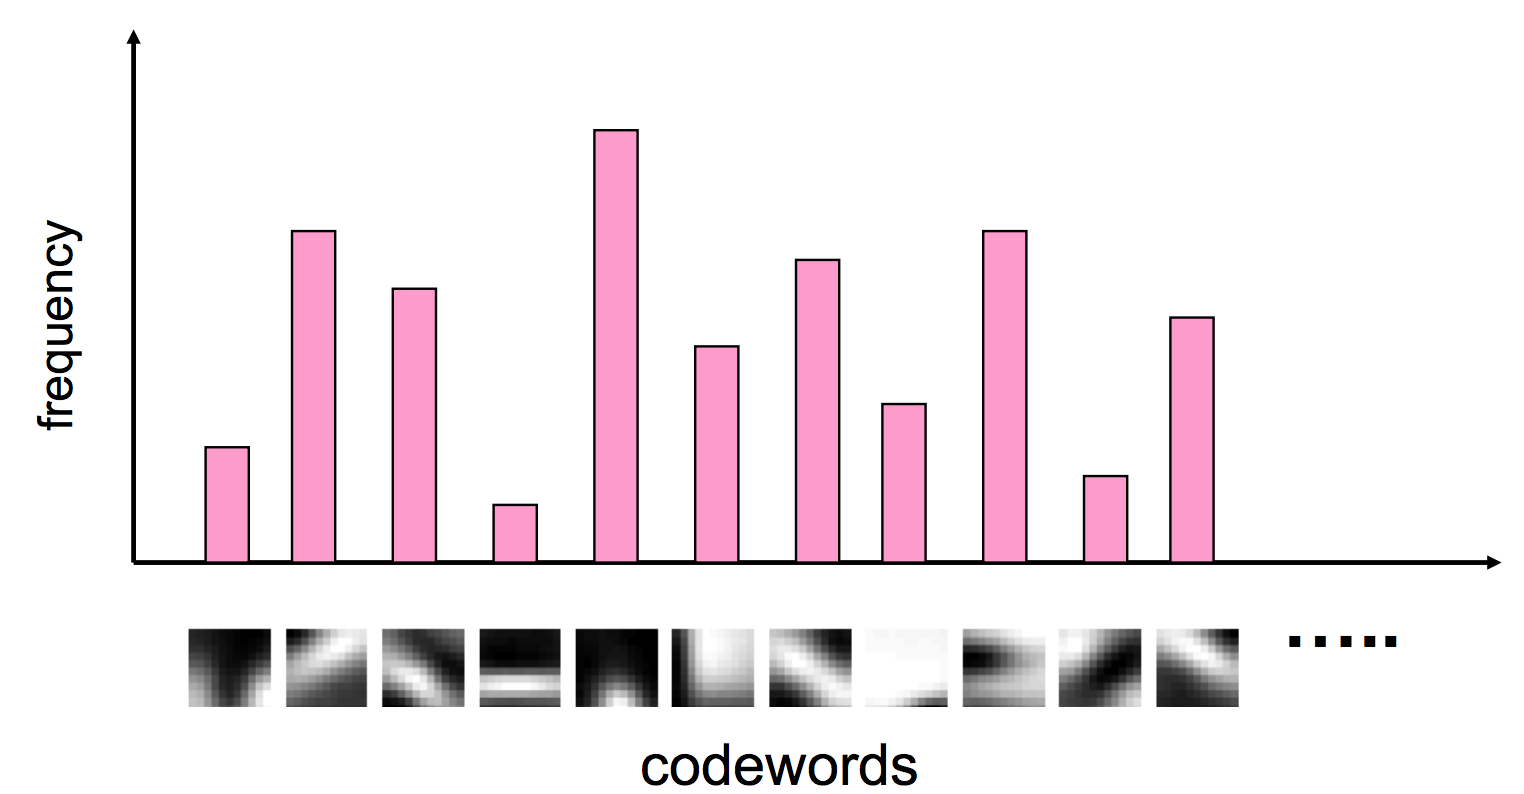
\includegraphics[scale=0.4]{hist.png}\\
Representing our images as a histogram of texton frequencies \cite{slides}
\end{center}

We can create our visual vocabulary from a different dataset than the dataset that we are interested in classifying/clustering, and so long as our first dataset is representative of the second, this algorithm will be successful.

\subsection{Large-Scale Image Search}
Large-scale image matching is one of the ways that the Bag-of-words model has been useful. Given a large database, which can hold tens of thousands of object instances, how can one match an images to this database?

The Bag-of-words model can help build the database.  First, features can be extracted from the database images. Then we can learn a vocabulary using k-means (typical k:100,000).  Next we compute the weights for each word.  Going back to the word dictionary example, weighting the words can help us decrease the importance of certain words.  If we are trying to find the topic of a document, we can give words like "the", "a", and "is" low weights since they are likely to be common between documents and used frequently within a document.  With images we can do the same, giving useless features low weights and the more important features higher weights.  Once the features have been weighted, we can create an inverted file mapping words to images.

Term Frequency Inverse Document Frequency (TF-IDF) scoring weights each word by it's document frequency.  

The inverse document frequency (IDF) of a word j can be found by

$$IDF = \log(\frac{NumDocs}{NumDocs_{j appears}})$$

To compute the value of bin j in image I:

$$Bin_{j} = frequncy_{j\,in\,I} * IDF$$

We can create an inverted file that holds the mapping of words to documents to quickly compute the similarity between a new image and all of the images in the database. If we have images that have around 1000 features, and a database of around 100,000 visual words, each histogram will be extremely sparse.  We would only consider images whose bins overlap with the new image.

Large-scale image search works well for CD covers and movie posters, and real-time performance is possible. The downside for the large scale image search is that the performance of the algorithm degrades as the database grows. Using the Bag-of-Words model for this problem sometimes results in noisy image similarities due to quantization error and imperfect feature detection.\cite{Large-scale-collections}
\section{Spatial Pyramid Matching}
\subsection{Motivation}
So far, we have not exploited the spatial information. But there is a simple yet smart method to incorporate the spatial information in the model: spatial pyramid matching.

\subsection{Pyramids}
A pyramid is built by using multiple copies	of the source image. Each level in the pyramid is $\frac{1}{4}$ of the size of the previous level. The lowest level is of the highest resolution and the highest level is of the lowest resolution. If illustrated graphically, the entire multi-scale representation looks like a pyramid, with the original image on the bottom and each cycle's resulting smaller image stacked one atop the other. {\cite{pyramid}}
\begin{center}
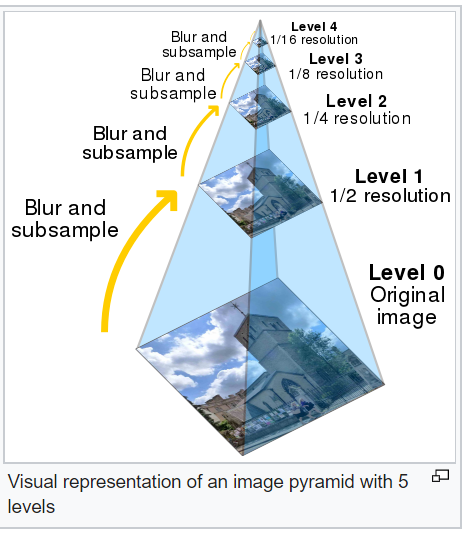
\includegraphics[width=8cm,height=6.4cm]{pyramid.PNG} 
\end{center}
\subsection{Bag of Words + Pyramids}
Bag of Words alone doesn't discriminate if a patch was obtained from the top, middle or bottom of the image because it doesn't save any spatial information. Spatial pyramid matching partitions the image into increasingly fine sub-regions and allows us to computes histograms (BoW) of local features inside each sub-region. \cite{quora}\\
If the BoWs of the upper part of the image contain "sky visual words", the BoWs in the middle "vegetation and mountains visual words" and the BoWs at the bottom "mountains visual words", then it is very likely that the image scene category is "mountains".
\begin{center}
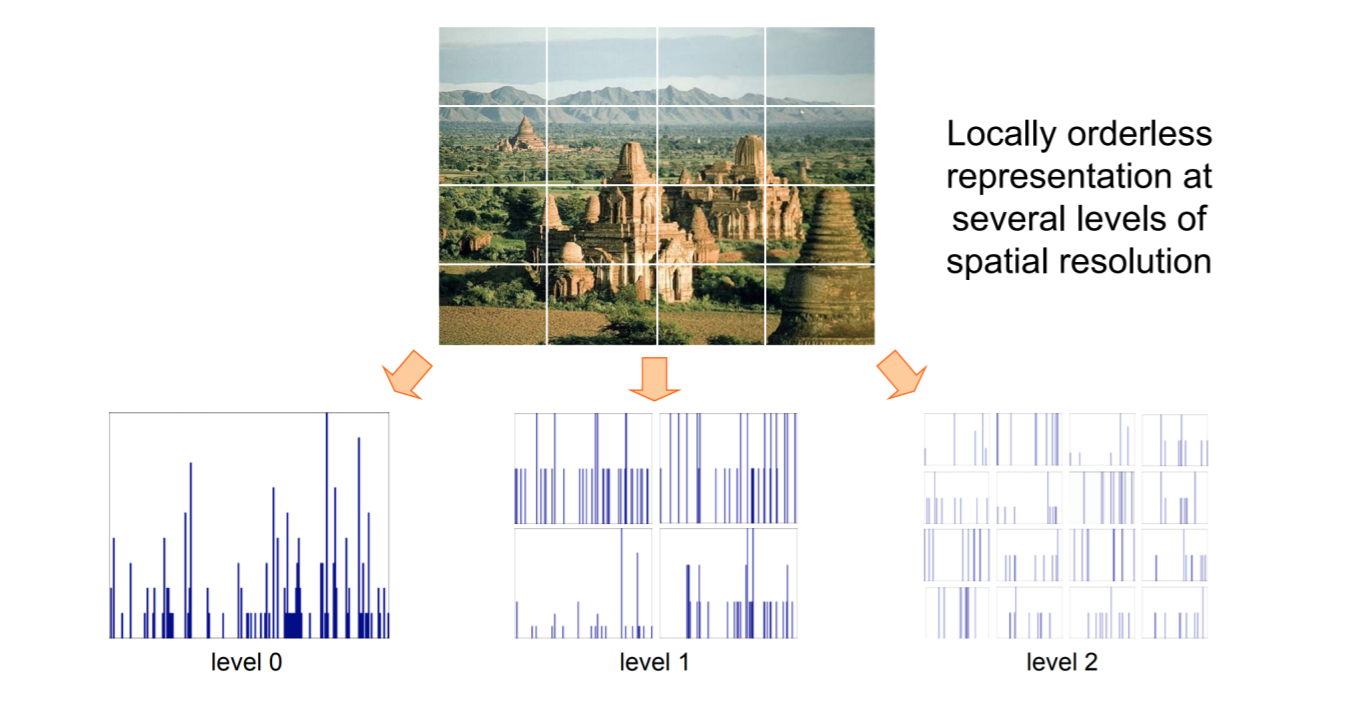
\includegraphics[width=10cm,height=6.4cm]{BoW_pyramid.PNG}
\end{center}
\subsection{Some results}
\begin{center}
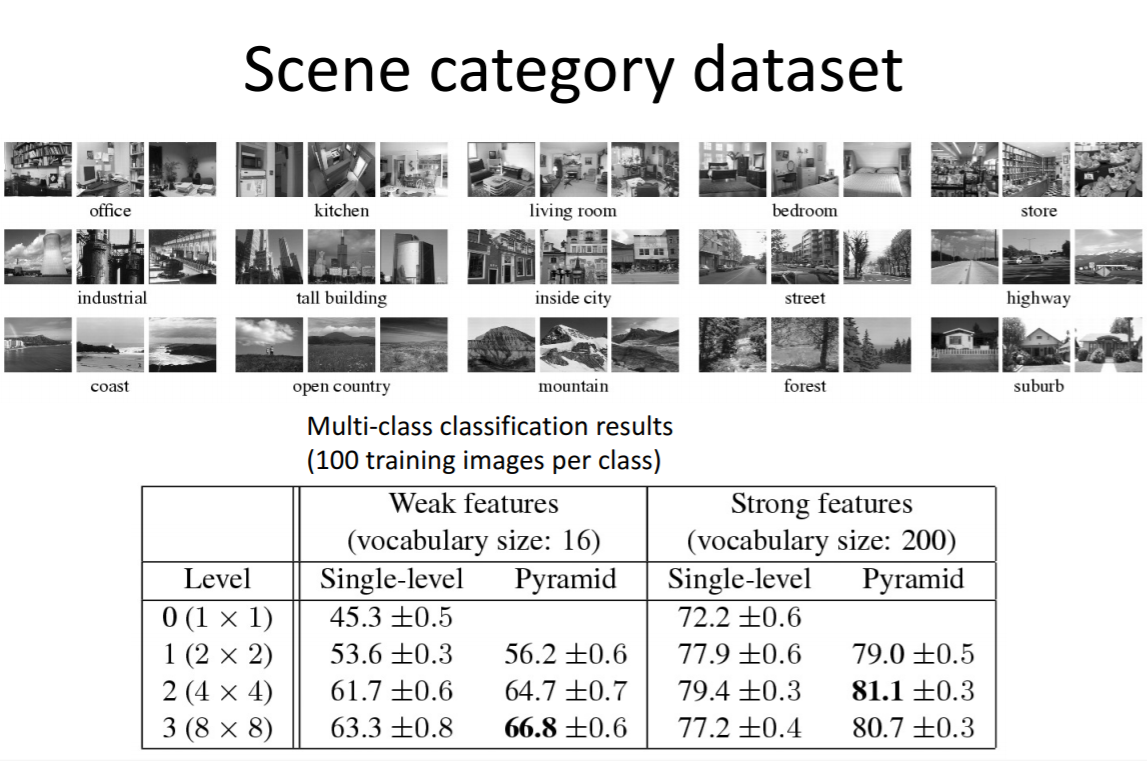
\includegraphics[width=10cm,height=6.4cm]{pyramid_data1.PNG}
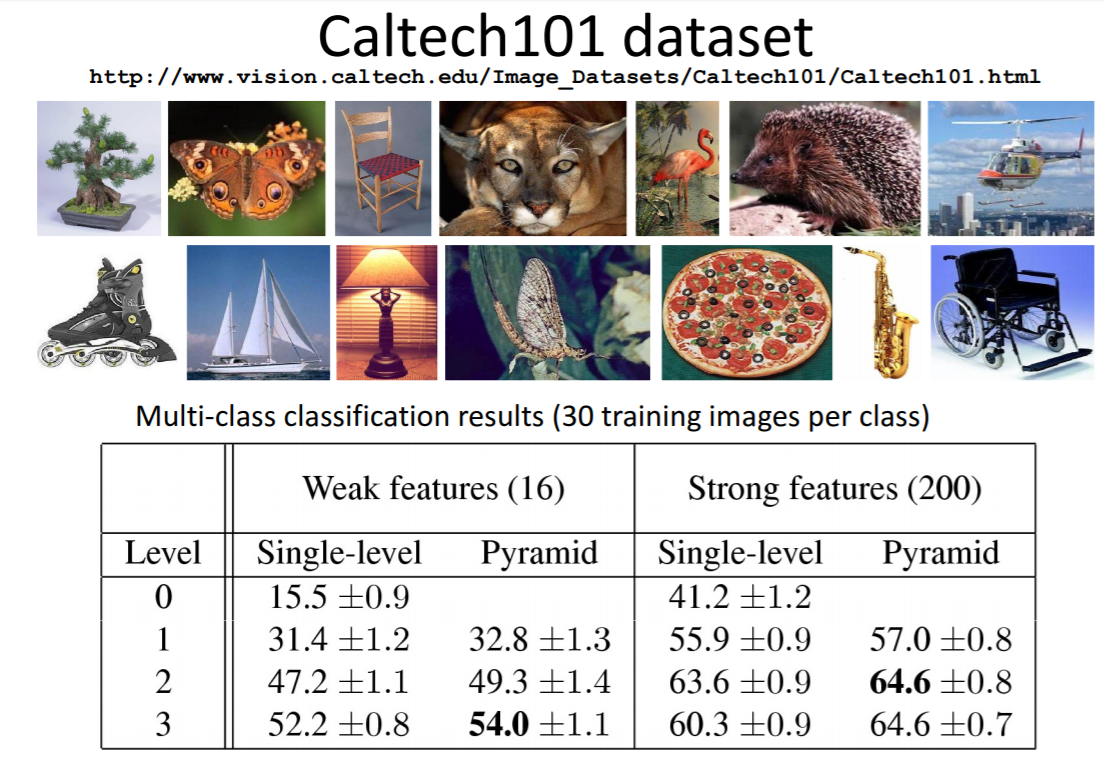
\includegraphics[width=10cm,height=6.4cm]{pyramid_data2.PNG}
\end{center}
Strong features (ie.larger vocabulary size) is better than weaker features (ie. smaller vocabulary size). Notice also that as expected, incorporating pyramid matching always generate better result than single level feature extraction. This is exactly what we expected because under the same circumstance, pyramid approach encodes more information (ie.spacial information) than single-level approach does.

\section{Naive Bayes}
\subsection{Basic Idea}
Once we have produced a visual word histogram, we can use Naive Bayes to classify the histogram. To do so, we simply measure whether a given visual word is present or absent, and assume the presence/absence of one visual word to be conditionally independent of each other visual word given an object class. 
\begin{center}
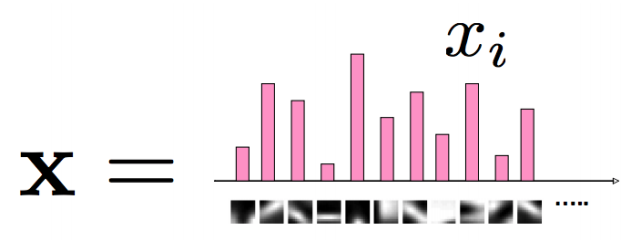
\includegraphics[width=10cm,height=4cm]{Bayes_Histogram}
\end{center}

Consider some visual word histogram \textit{X}, where $x_i$ is the count of visual word \textit{i} in the histogram. We are only interested in the presence or absence of word \textit{i}, we have $x_i \in \{0,1\}$.  
\subsection{Prior}
$P(c)$ denotes that probability of encountering one object class versus others. For all $m$ object classes, we then have $$\sum_{i=1}^m P(c)=1$$ For an image represented by histogram $x$, and some object class $c$, we can compute $$P(x|c) = \prod_{i=1}^m P(x_i|c)$$
We are able to make the above statement by assuming the mutual independence of each feature $x_i$ when conditioned on $c$. This assumption is called the Naive Bayes Assumption.
\subsection{Posterior}
Using the prior equation, we can now calculate the probability than the image represented by histogram $x$ belongs to class category $c$ using \textbf{Bayes Theorem}. $$P(c|x) = \frac{P(c)P(x|c)}{\sum_{c'}P(c')P(x|c')}$$
Note that we express $P(x)$ as the summation of $P(c')P(x|c')$, or equivalently $P(x,c')$ for all $c'$ by using the law of total probability. Expanding the numerator and denominator, we can rewrite the previous equation as 
$$P(c|x) = \frac{P(c)\prod_{i=1}^mP(x_i|c)}{\sum_{c'}P(c')\prod_{i=1}^mP(x_i|c')}$$ by once again using the Naive Bayes Assumption of conditional independence of each $x_i$ on $c'$.
\subsection{Classification}
In order to classify the image represented by histogram $x$, we simply find the class $c^*$ that maximizes the previous equation. That is to say, we look for the label $c = c^*$ such that the label that $c$ has the highest probability of taking on given its feature data is $c^*$:
$$c^*=arg{max}_{c}P(c|x)$$
Since we end up multiplying together a large number of very small probabilities, we will likely run into unstable values as they approach 0. As a result, we use logs to calculate probabilities:
$$c^*=arg{max}_{c}logP(c|x)$$
Now consider two classes $c_1$ and $c_2$:
$$P(c_1|x) = \frac{P(c_1)\prod_{i=1}^mP(x_i|c_1)}{\sum_{c'}P(c')\prod_{i=1}^mP(x_i|c')}$$
and
$$P(c_2|x) = \frac{P(c_2)\prod_{i=1}^mP(x_i|c_2)}{\sum_{c'}P(c')\prod_{i=1}^mP(x_i|c')}$$
Since the denominators are identical, we can ignore it when calculating the maximum. Thus
$$P(c_1|x) \propto P(c_1)\prod_{i=1}^mP(x_i|c_1)$$
and
$$P(c_2|x) \propto P(c_2)\prod_{i=1}^mP(x_i|c_2)$$
and for the general class $c$:
$$P(c|x) \propto P(c)\prod_{i=1}^mP(x_i|c)$$
and using logs:
$$logP(c|x) \propto logP(c)+\sum_{i=1}^mlogP(x_i|c)$$

Now, classification becomes 
$$c^*=arg{max}_{c}P(c|x)$$
$$c^*=arg{max}_{c}logP(c|x)$$
$$c^*=arg{max}_{c}logP(c)+\sum_{i=1}^mlogP(x_i|c)$$

% References
%{\small
%\bibliographystyle{plain}
%\bibliography{bibliography.bib}
%}

\end{document}